% report.tex — Отчёт по учебной практике
% Оформление по ГОСТ 7.32-2017
\documentclass[a4paper,14pt]{extarticle}

% preamble.tex — Преамбула отчёта по практике
% Оформление по ГОСТ 7.32-2017

\usepackage[T2A]{fontenc}
\usepackage[utf8]{inputenc}
\usepackage[english,russian]{babel}

\usepackage{mathptmx}                        % Times New Roman

\usepackage[nodisplayskipstretch]{setspace}   % Полуторный интервал
\onehalfspacing

% Поля: лев 30, прав 15, верх 20, низ 20 мм
\usepackage[top=20mm, bottom=20mm, left=30mm, right=15mm]{geometry}

\parindent=1.25cm
\usepackage{indentfirst}

% Нумерация страниц в правом верхнем углу
\usepackage{fancyhdr}
\pagestyle{fancy}
\fancyhf{}
\fancyhead[R]{\thepage}
\renewcommand{\headrulewidth}{0pt}
\renewcommand{\footrulewidth}{0pt}
\fancypagestyle{plain}{
  \fancyhf{}
  \fancyhead[R]{\thepage}
  \renewcommand{\headrulewidth}{0pt}
  \renewcommand{\footrulewidth}{0pt}
}

% Содержание
\usepackage{titletoc}
\usepackage{tocloft}
\usepackage{etoolbox}
\setcounter{tocdepth}{3}

\makeatletter
\patchcmd{\@cftmaketoctitle}{\cfttoctitlefont\contentsname}{\cfttoctitlefont\MakeUppercase{\contentsname}}{}{}
\makeatother

\renewcommand{\cftsecleader}{\cftdotfill{\cftdotsep}}

% Заголовки: с абзацного отступа, полужирный
\usepackage{titlesec}
\usepackage{textcase}

\titleformat{\section}[block]{\hspace{\parindent}\bfseries\normalsize}
                         {\arabic{section}}{1ex}{\MakeUppercase}
\titlespacing*{\section}{0pt}{42pt}{42pt}

\titleformat{\subsection}[block]{\hspace{\parindent}\bfseries\normalsize}
                         {\arabic{section}.\arabic{subsection}}{1ex}{}
\titlespacing*{\subsection}{0pt}{\baselineskip}{\baselineskip}

\titleformat{\subsubsection}[block]{\hspace{\parindent}\bfseries\normalsize}
                         {\arabic{section}.\arabic{subsection}.\arabic{subsubsection}}{1ex}{}
\titlespacing*{\subsubsection}{0pt}{\baselineskip}{\baselineskip}

% Подписи: разделитель — короткое тире
\usepackage{caption}
\DeclareCaptionLabelSeparator{endash}{ -- }
\captionsetup{labelsep=endash}
\captionsetup[figure]{justification=centering, font=normalsize}
\captionsetup[table]{singlelinecheck=false, justification=raggedright, font=normalsize}

\addto\captionsrussian{
  \def\figurename{Рисунок}
  \def\tablename{Таблица}
  \def\contentsname{Содержание}
  \def\refname{СПИСОК ИСПОЛЬЗОВАННЫХ ИСТОЧНИКОВ}
}

% Сквозная нумерация
\renewcommand{\theequation}{\arabic{equation}}
\renewcommand{\thetable}{\arabic{table}}
\renewcommand{\thefigure}{\arabic{figure}}

\usepackage{amsmath}
\usepackage{amssymb}

\usepackage{graphicx}
\graphicspath{{images/}}
\usepackage{float}

\usepackage{multirow}
\usepackage{longtable}
\usepackage{booktabs}
\usepackage{array}

% Списки: маркер — тире
\usepackage{enumitem}
\setlist[enumerate]{topsep=0pt, itemsep=0ex, partopsep=1ex, parsep=1ex}
\setlist[itemize]{topsep=0pt, itemsep=0ex, partopsep=1ex, parsep=1ex}
\def\labelitemi{--}

% Листинги кода с поддержкой кириллицы
\usepackage{listings}
\usepackage{xcolor}
\lstset{
  basicstyle=\small\ttfamily,
  breaklines=true,
  frame=single,
  xleftmargin=\parindent,
  showstringspaces=false,
  extendedchars=true,
  literate=
    {а}{{\cyra}}1 {б}{{\cyrb}}1 {в}{{\cyrv}}1 {г}{{\cyrg}}1
    {д}{{\cyrd}}1 {е}{{\cyre}}1 {ё}{{\cyryo}}1 {ж}{{\cyrzh}}1
    {з}{{\cyrz}}1 {и}{{\cyri}}1 {й}{{\cyrishrt}}1 {к}{{\cyrk}}1
    {л}{{\cyrl}}1 {м}{{\cyrm}}1 {н}{{\cyrn}}1 {о}{{\cyro}}1
    {п}{{\cyrp}}1 {р}{{\cyrr}}1 {с}{{\cyrs}}1 {т}{{\cyrt}}1
    {у}{{\cyru}}1 {ф}{{\cyrf}}1 {х}{{\cyrh}}1 {ц}{{\cyrc}}1
    {ч}{{\cyrch}}1 {ш}{{\cyrsh}}1 {щ}{{\cyrshch}}1 {ъ}{{\cyrhrdsn}}1
    {ы}{{\cyrery}}1 {ь}{{\cyrsftsn}}1 {э}{{\cyrerev}}1 {ю}{{\cyryu}}1
    {я}{{\cyrya}}1
    {А}{{\CYRA}}1 {Б}{{\CYRB}}1 {В}{{\CYRV}}1 {Г}{{\CYRG}}1
    {Д}{{\CYRD}}1 {Е}{{\CYRE}}1 {Ё}{{\CYRYO}}1 {Ж}{{\CYRZH}}1
    {З}{{\CYRZ}}1 {И}{{\CYRI}}1 {Й}{{\CYRISHRT}}1 {К}{{\CYRK}}1
    {Л}{{\CYRL}}1 {М}{{\CYRM}}1 {Н}{{\CYRN}}1 {О}{{\CYRO}}1
    {П}{{\CYRP}}1 {Р}{{\CYRR}}1 {С}{{\CYRS}}1 {Т}{{\CYRT}}1
    {У}{{\CYRU}}1 {Ф}{{\CYRF}}1 {Х}{{\CYRH}}1 {Ц}{{\CYRC}}1
    {Ч}{{\CYRCH}}1 {Ш}{{\CYRSH}}1 {Щ}{{\CYRSHCH}}1 {Ъ}{{\CYRHRDSN}}1
    {Ы}{{\CYRERY}}1 {Ь}{{\CYRSFTSN}}1 {Э}{{\CYREREV}}1 {Ю}{{\CYRYU}}1
    {Я}{{\CYRYA}}1,
}

\usepackage{hyperref}
\hypersetup{unicode=true, colorlinks=false, pdfborder={0 0 0}}
\expandafter\def\expandafter\UrlBreaks\expandafter{\UrlBreaks
  \do\a\do\b\do\c\do\d\do\e\do\f\do\g\do\h\do\i\do\j
  \do\k\do\l\do\m\do\n\do\o\do\p\do\q\do\r\do\s\do\t
  \do\u\do\v\do\w\do\x\do\y\do\z\do\A\do\B\do\C\do\D
  \do\E\do\F\do\G\do\H\do\I\do\J\do\K\do\L\do\M\do\N
  \do\O\do\P\do\Q\do\R\do\S\do\T\do\U\do\V\do\W\do\X
  \do\Y\do\Z}

\usepackage{cmap}
\usepackage{pdfpages}

\usepackage[numbers,sort&compress]{natbib}
\makeatletter
\renewcommand\@biblabel[1]{#1.}
\makeatother

\tolerance 1414
\hbadness 1414
\emergencystretch 1.5em
\hfuzz 0.3pt
\widowpenalty=10000
\vfuzz \hfuzz
\raggedbottom


\begin{document}

% === ТИТУЛЬНЫЙ ЛИСТ ===
\begin{titlepage}
\thispagestyle{empty}
\vspace{4pt}
\begin{center}
Министерство науки и высшего образования Российской Федерации\\
\textbf{ФЕДЕРАЛЬНОЕ ГОСУДАРСТВЕННОЕ АВТОНОМНОЕ ОБРАЗОВАТЕЛЬНОЕ УЧРЕЖДЕНИЕ ВЫСШЕГО ОБРАЗОВАНИЯ}\\
\textbf{<<НАЦИОНАЛЬНЫЙ ИССЛЕДОВАТЕЛЬСКИЙ УНИВЕРСИТЕТ ИТМО>>}\\
\textbf{(Университет ИТМО)}\\[8pt]
\textbf{Факультет программной инженерии и компьютерной техники}
\end{center}
\vspace{10pt}
Образовательная программа \underline{Компьютерные системы и технологии}\\[6pt]
Направление подготовки (специальность) \\
\underline{09.03.01 --- Информатика и вычислительная техника}\\[18pt]
\begin{center}
{\large \textbf{О Т Ч Ё Т}}\\[6pt]
об учебной практике
\end{center}
\vspace{12pt}
Тема задания: \underline{Проектная документация}\\[10pt]
Обучающийся: \underline{Нодири Хисравхон}, № группы \underline{P3431}\\[12pt]
Руководитель практики от университета:\\
\underline{Маркина Татьяна Анатольевна, старший преподаватель}\\
\hspace*{8cm}(Ф.И.О., должность)\\[14pt]
Практика пройдена с оценкой \underline{\hspace{2cm}}\\[12pt]
Дата \underline{11.02.2026}
\vfill
\begin{center}
Санкт-Петербург\\
2026 г.
\end{center}
\end{titlepage}

% === СОДЕРЖАНИЕ ===
\thispagestyle{fancy}
\tableofcontents
\newpage

% === СПИСОК СОКРАЩЕНИЙ И УСЛОВНЫХ ОБОЗНАЧЕНИЙ ===
\phantomsection
\begin{center}
\textbf{СПИСОК СОКРАЩЕНИЙ И УСЛОВНЫХ ОБОЗНАЧЕНИЙ}
\end{center}
\addcontentsline{toc}{section}{СПИСОК СОКРАЩЕНИЙ И УСЛОВНЫХ ОБОЗНАЧЕНИЙ}

\noindent
ВКР -- выпускная квалификационная работа\\
ГОСТ -- государственный стандарт\\
ЕСПД -- единая система программной документации\\
ПО -- программное обеспечение\\
ТЗ -- техническое задание\\
ИТМО -- Национальный исследовательский университет информационных технологий, механики и оптики\\
ПИиКТ -- факультет программной инженерии и компьютерной техники

\newpage

% === ВВЕДЕНИЕ ===
\phantomsection
\begin{center}
\textbf{ВВЕДЕНИЕ}
\end{center}
\addcontentsline{toc}{section}{ВВЕДЕНИЕ}

Тема учебной практики: Проектная документация.

Цель: приобретение навыков подготовки проектной документации для выпускной квалификационной работы в соответствии с требованиями Университета ИТМО и действующими стандартами.

Задачи практики:
\begin{enumerate}
  \item посетить лекционные занятия и изучить требования к оформлению документации;
  \item подготовить шаблон для ВКР;
  \item написать техническое задание по ВКР;
  \item оформить отчёт по практике.
\end{enumerate}

Выполнение практики состоит из прохождения этапов, приведённых в таблице~\ref{tab:stages}.

\begin{table}[H]
\caption{Этапы учебной практики}
\label{tab:stages}
\centering
\small
\begin{tabular}{|c|p{3.5cm}|p{9.5cm}|}
\hline
\textbf{№ этапа} & \textbf{Название этапа} & \textbf{Задание} \\ \hline
1 & Инструктаж обучающегося & Инструктаж обучающегося по ознакомлению с требованиями охраны труда, техники безопасности, пожарной безопасности, а также правилами внутреннего трудового распорядка \\ \hline
2 & Лекции & Посетить 2 занятия \\ \hline
3 & Шаблон для ВКР & Подготовить шаблон для ВКР по требованиям университета. Создать шаблоны шрифтов, задать структуру ВКР. Прислать сформированный на основе шаблона текстовый документ в формате doc или txt, или подготовленный шаблона в LateX или Typst. Задание выполняется полностью самостоятельно, без использования заготовок. Сформировать документ или архив и прислать на проверку на электронную почту преподавателя. \\ \hline
4 & Техническое задание по ВКР & Написать техническое задание по ВКР. Техническое задание должно содержать: наименование, назначение, основание для разработки, функции, структура, пользовательский интерфейс, требования к надёжности, требования к безопасности, условия эксплуатации и проч. важные требования, документация, стадии и этапы разработки, порядок контроля и приёмка. В случае отсутствия какого-либо пункта необходимо обосновать его отсутствие. Сформировать в виде документа в формате pdf и прислать на проверку на электронную почту преподавателя. \\ \hline
5 & Оформление отчётных документов в соответствии с требованиями & 1. Должно быть подробное описание выполнения задач по этапам. Результаты задания необходимо разместить в приложения. 2. Оформление отчёта должно быть выполнено в соответствии с методическим пособием (https://books.ifmo.ru/file/pdf/2622.pdf) 3. Структура документа: титульный лист, введение, основная часть, заключение, приложения. 4. В основной части подробно описывается выполнение задач 2-4 этапов, в приложении помещаются результаты данных этапов. 5. Отчёт необходимо подгрузить в модуле практика как "письменный отчёт" \\ \hline
6 & Получение отзыва руководителя практики & Получить отзыв с оценкой у руководителя практики в модуле Практики \\ \hline
\end{tabular}
\end{table}

В основной части отчёта подробно описывается выполнение этапов 2--4. Результаты этапов размещены в приложениях.

Место прохождения практики~--- Федеральное государственное автономное образовательное учреждение высшего образования <<Национальный исследовательский университет ИТМО>>, факультет программной инженерии и компьютерной техники.

Сроки прохождения практики: 04.02.2026~-- 11.02.2026.

\newpage

% === ГЛАВА 2: ЛЕКЦИИ (ЭТАП 2) ===
\section{Лекции}

В рамках второго этапа практики необходимо было посетить два лекционных занятия.

\subsection{Подготовка к участию в практике}

02.02.2026 в Telegram-канале практики группы было опубликовано объявление о начале проведения учебной практики с 04.02.2026. Было указано проведение онлайн-занятий, проведён опрос предпочтительного времени (8:20, 18:50). В голосовании выбрал время 18:50.

04.02.2026 опубликована информация о проведении занятий:
\begin{itemize}
  \item укороченные лекции №1 и №2: 05.02.2026, 18:50 (КТолк-комната);
  \item консультация: 10.02.2026;
  \item инструкция по заполнению индивидуального задания практики на my.itmo.
\end{itemize}

Открыл прикреплённую инструкцию (PDF), следуя ей, перешёл на my.itmo $\rightarrow$ Практики $\rightarrow$ Учебная практика $\rightarrow$ Индивидуальное задание. В соответствии с инструкцией в сообщении заполнил:
\begin{itemize}
  \item тему задания: <<Проектная документация>>;
  \item заполнил этапы по инструкции.
\end{itemize}

Сохранил черновик, решил отправить позже --- 05.02.2026, чтобы узнать о потенциальных ошибках. Для этого просматривал чат группы (у некоторых студентов была проблема с датами, у меня не возникло).

\subsection{Лекционный день}

05.02.2026 в Telegram-канале и на почте были опубликованы ссылки на КТолк-комнату. На лекцию присутствовать не смог по личным обстоятельствам. Поскольку было объявлено, что лекция будет записана, решил посмотреть запись позже.

\subsection{Просмотр записи лекции}

06.02.2026 в Telegram-канале опубликована запись лекции. Просмотрел её полностью, так как не присутствовал на занятии лично. При просмотре вёл заметки, выделяя ключевые требования к выполнению заданий этапов 3 и 4.

Основные тезисы лекции:
\begin{itemize}
  \item условия прохождения практики и требования к отчётности;
  \item проектная документация: ТЗ составляется на <<проект <<Написание ВКР>>>>, а не на программное обеспечение (ключевой момент для этапа~4);
  \item шаблон ВКР (этап~3): открыл ссылки, отправленные в чат КТолк-комнаты во время лекции;
  \item источники: 20--40 штук, 2/3 не старше 2022 года, исходный код только в приложения (не ссылки);
  \item отчёт по практике: подробно описывать процесс по этапам, результат 4-го этапа размещать в приложениях.
\end{itemize}

Также обратил внимание на вопросы студентов и ответы преподавателя:
\begin{itemize}
  \item основания для разработки ТЗ --- устав ИТМО, ГОСТы, требования к ВКР, документации, гайдлайны, а также любые письменные элементы, относящиеся к работе над ВКР;
  \item приложение датасетов --- необходимо, если они не опубликованы, иначе можно сослаться на источник.
\end{itemize}

Найденные требования к ТЗ (этап~4):
\begin{itemize}
  \item обязательная структура: наименование, назначение разработки, основания для разработки, функции (очевидные и неочевидные), структура проекта, пользовательский интерфейс, дополнительные требования (надежность, безопасность...), документация, стадии/этапы, порядок контроля;
  \item <<разрабатываемое ПО>> заменить на <<проект <<Написание ВКР>>>>;
  \item ТЗ отправлять только в PDF.
\end{itemize}

Найденные требования к шаблону ВКР (этап~3):
\begin{itemize}
  \item форматы: Word (.doc/.docx) или \LaTeX{} (.zip с исходниками и собранным PDF);
  \item требования к оформлению и содержанию ВКР: <<ТРЕБОВАНИЯ К ВЫПУСКНЫМ КВАЛИФИКАЦИОННЫМ РАБОТАМ>> ЛНАОБУЧ-СМК-03-05-2022;
  \item результат этапа~3 не включается в отчёт по практике.
\end{itemize}

Выводы для планирования:
\begin{itemize}
  \item этап~3 необходимо выполнить перед этапом~4, т.к. ТЗ включает структуру разработанного шаблона ВКР.
\end{itemize}

Детальный разбор использован при выполнении этапов 3 и 4.

\subsection{Консультация (второе занятие)}

10.02.2026 состоялось второе занятие --- консультация. Подключился к КТолк-комнате, переименовался в <<Нодири Хисравхон P3431>>, сделал скриншот присутствия (приложение~А).

На консультации руководитель практики разбирала отчёты студентов, указывая на типичные ошибки. Зафиксировал для себя следующие замечания:
\begin{itemize}
  \item описание этапов должно содержать не пересказ лекции, а действия студента: что делал, зачем, почему именно так;
  \item каждый выбор (инструмент, формат, структура) необходимо обосновать;
  \item если трудностей не возникло, это тоже следует отметить;
  \item завершением этапа считается получение оценки от руководителя;
  \item скриншоты присутствия необходимы с обоих занятий (5-го и 10-го числа);
  \item нумерация страниц в отчёте должна быть сквозной, включая приложения.
\end{itemize}

После консультации доработал отчёт с учётом полученных замечаний: добавил обоснования принятых решений, описание трудностей и результатов каждого этапа.

\newpage

% === ГЛАВА 3: ШАБЛОН ДЛЯ ВКР (ЭТАП 3) ===
\section{Шаблон для ВКР}

\subsection{Сбор требований}

06.02.2026 --- пересмотрел запись лекции и нашёл конкретные требования к шаблону ВКР (см.~2.3). Также прочел требования к оформлению ВКР по документу ЛНАОБУЧ-СМК-03-05-2022~\cite{gost732}:
\begin{itemize}
  \item нумерация страниц;
  \item структурные элементы, заголовки, подзаголовки;
  \item иллюстрации/таблицы/формулы;
  \item списки сокращений/терминов/источников;
  \item приложения.
\end{itemize}

Прочел вопросы преподавателю из чата и ответы на них, получив следующую информацию:
\begin{itemize}
  \item требуется написать только текст ВКР;
  \item текстовые заглушки разрешены.
\end{itemize}

\subsection{Выбор инструмента}

В качестве инструмента для подготовки шаблона выбрал систему вёрстки \LaTeX{}~\cite{latex_project}. Выбор обусловлен следующими причинами:
\begin{itemize}
  \item автоматическая нумерация разделов, рисунков, таблиц;
  \item автоматическое формирование содержания и списка литературы;
  \item высокое качество типографского набора;
  \item удобство версионного контроля (текстовые исходники)~\cite{lvovsky2003}.
\end{itemize}

Использовал класс документа \texttt{extarticle} с параметром 14~пт --- стандартные классы \LaTeX{} не поддерживают размер 14~пт, поэтому применение расширенного класса является обязательным.

\subsection{Настройка преамбулы}

Создал файл \texttt{preamble.tex} с настройками оформления. Последовательность действий:

\begin{enumerate}
  \item Подключил пакеты кодировки: \texttt{fontenc} (T2A), \texttt{inputenc} (utf8), \texttt{babel} (english, russian) --- для корректного отображения кириллицы.
  \item Подключил пакет \texttt{mathptmx} --- замена стандартного шрифта на Times New Roman~\cite{kotelnikov2004}.
  \item Настроил поля через пакет \texttt{geometry}: левое --- 30~мм, правое --- 15~мм, верхнее и нижнее --- 20~мм.
  \item Задал полуторный интервал: пакет \texttt{setspace}, команда \texttt{\textbackslash onehalfspacing}.
  \item Установил абзацный отступ 1,25~см: \texttt{\textbackslash parindent=1.25cm}, пакет \texttt{indentfirst}.
  \item Настроил нумерацию страниц по центру внизу: пакет \texttt{fancyhdr}, убрал линии-разделители.
  \item Настроил заголовки разделов через пакет \texttt{titlesec}: разделы --- прописными буквами, полужирный, с отступа; подразделы --- строчными, полужирный, с отступа.
  \item Настроил подписи рисунков и таблиц: пакет \texttt{caption}, разделитель <<~--~>> (короткое тире).
  \item Переопределил названия: <<Рисунок>>, <<Таблица>>, <<Содержание>>.
  \item Подключил пакет \texttt{listings} для листингов кода с поддержкой кириллицы через механизм \texttt{literate}.
  \item Настроил список литературы: пакет \texttt{natbib}, стиль \texttt{unsrtnat} --- нумерация в порядке первого упоминания~\cite{gost71}.
\end{enumerate}

\subsection{Формирование структуры документа}

Создал основной файл шаблона \texttt{vkr.tex}. Включил следующие структурные элементы:
\begin{enumerate}
  \item титульный лист (закомментированный вариант, т.к. оформляется в ИСУ);
  \item содержание (автоматическое через \texttt{\textbackslash tableofcontents});
  \item список сокращений и условных обозначений;
  \item термины и определения;
  \item введение;
  \item три раздела основной части с примерами подразделов и пунктов;
  \item заключение;
  \item список использованных источников (из BibTeX-базы);
  \item приложения А и Б.
\end{enumerate}

В каждом разделе предусмотрел примеры: рисунок с подписью и ссылкой, таблица, маркированный список, листинг кода на Python.

\subsection{Создание файла библиографии}

Создал файл \texttt{references.bib} с примерами записей различных типов источников:
\begin{itemize}
  \item ГОСТ (тип \texttt{misc});
  \item книга (тип \texttt{book});
  \item статья в журнале (тип \texttt{article});
  \item веб-сайт (тип \texttt{misc} с полем \texttt{howpublished});
  \item диссертация (тип \texttt{phdthesis});
  \item доклад на конференции (тип \texttt{inproceedings}).
\end{itemize}

\subsection{Тестирование и отправка}

Скомпилировал шаблон командами:
\begin{enumerate}
  \item \texttt{pdflatex vkr.tex} --- первый проход (формирование aux-файла);
  \item \texttt{bibtex vkr} --- обработка библиографии;
  \item \texttt{pdflatex vkr.tex} --- второй проход (подстановка ссылок);
  \item \texttt{pdflatex vkr.tex} --- третий проход (финализация содержания).
\end{enumerate}

Проверил результат:
\begin{itemize}
  \item корректность отображения кириллического текста;
  \item соответствие полей, шрифта, интервала требованиям;
  \item автоматическая нумерация разделов, рисунков, таблиц;
  \item формирование содержания и списка литературы;
  \item корректность перекрёстных ссылок;
  \item отображение листингов кода с кириллицей.
\end{itemize}

Ошибок не обнаружено. Существенных трудностей при выполнении этапа не возникло, поскольку ранее имел опыт работы с \LaTeX{}.

Сформировал архив (.zip) с исходниками и собранным PDF, направил на проверку руководителю практики на электронную почту. По результатам проверки получил оценку.

\newpage

% === ГЛАВА 4: ТЕХНИЧЕСКОЕ ЗАДАНИЕ ПО ВКР (ЭТАП 4) ===
\section{Техническое задание по ВКР}

\subsection{Подготовка}

07.02.2026 --- пересмотрел запись лекции и выделил требования к оформлению ТЗ (см.~2.3). Начал искать требования в ГОСТ~34 и ГОСТ~19, нашёл ГОСТ~19.201-78~\cite{gost19201}, в котором описывается содержание ТЗ. Связанные ГОСТы также посмотрел~\cite{gost34602}, но не нашёл требований к оформлению, в связи с чем решил придерживаться стилей шаблона ВКР.

\subsection{Создание документа}

Выполнил действия аналогично пункту~3.2: создал новый \LaTeX{}-документ с подключением \texttt{preamble.tex} из шаблона ВКР. Это обеспечило единообразие оформления ТЗ и будущей ВКР.

\subsection{Написание разделов}

Создал необходимые стили по аналогии с пунктом~3.3. Написал все обязательные разделы ТЗ согласно структуре (пункт~2.3): наименование, назначение, основания, функции, структура, пользовательский интерфейс, требования, документация, этапы, контроль.

Особенности работы над разделами:
\begin{itemize}
  \item введение и назначение: связал тему ВКР с проектом <<Написание ВКР>>, развёл <<для чего>> (цикл работ по ВКР) и <<зачем>> (ГИА, компетенции);
  \item основания для разработки: перечислил документы --- ЛНАОБУЧ-СМК-03-04/05-2022, учебный план ОП 09.03.01, задание практики, утверждённую тему ВКР;
  \item функции проекта: описал типы функций (планирующая, организационная, информационно-поисковая, письменная, документационная, коммуникационная) согласно требованию <<очевидные и неочевидные>> из лекции;
  \item структура: использовал готовую структуру из шаблона ВКР;
  \item пользовательский интерфейс: определил пользователей (студент, руководитель) и формат (PDF ВКР) с требованиями к оформлению;
  \item требования к надёжности: описал резервное копирование, контроль версий;
  \item требования к безопасности: описал проверку на заимствования (Антиплагиат);
  \item этапы, контроль: подробно расписал согласно организационному собранию --- график работ, этапы проверок 0--2, Антиплагиат, ГЭК.
\end{itemize}

\subsection{Оформление и отправка}

Скомпилировал документ аналогично пункту~3.6. Проверил:
\begin{itemize}
  \item наличие всех обязательных разделов;
  \item корректность ссылок на ГОСТы и нормативные документы;
  \item единообразие оформления с шаблоном ВКР.
\end{itemize}

Трудностей при оформлении не возникло, так как стили были перенесены из шаблона ВКР (этап~3). Основная сложность заключалась в формулировании содержания разделов --- необходимо было адаптировать структуру ТЗ на программное обеспечение к проекту <<Написание ВКР>>.

Сформировал документ в формате PDF и направил на проверку руководителю практики по электронной почте. По результатам проверки получил оценку.

Результат выполнения данного этапа (техническое задание) представлен в Приложении~Б.

\newpage

% === ЗАКЛЮЧЕНИЕ ===
\phantomsection
\begin{center}
\textbf{ЗАКЛЮЧЕНИЕ}
\end{center}
\addcontentsline{toc}{section}{ЗАКЛЮЧЕНИЕ}

В ходе прохождения учебной практики были выполнены все этапы, предусмотренные индивидуальным заданием.

На этапе посещения лекций (этап~2) лекция 05.02.2026 была просмотрена в записи, консультация 10.02.2026 посещена лично. Получены теоретические знания о требованиях к оформлению отчётных документов, стандартах проектной документации и типовых ошибках. Запись лекции была детально разобрана для выделения конкретных требований к этапам 3 и~4. На консультации зафиксированы замечания по типичным ошибкам в отчётах, которые были учтены при доработке.

На этапе подготовки шаблона для ВКР (этап~3) был разработан шаблон в системе \LaTeX{}, включающий настройку шрифтов, полей, интервалов, заголовков, подписей рисунков и таблиц, списка литературы и листингов кода. Шаблон обеспечивает автоматическое соблюдение требований ГОСТ~7.32-2017~\cite{gost732} и ЛНАОБУЧ-СМК-03-05-2022.

На этапе разработки технического задания (этап~4) было составлено ТЗ на проект <<Написание ВКР>> в соответствии с ГОСТ~19.201-78~\cite{gost19201}. ТЗ содержит все обязательные разделы, оформлено с использованием стилей шаблона ВКР.

На этапе оформления отчётных документов (этап~5) был подготовлен настоящий отчёт в соответствии с методическим пособием~\cite{markina2020}.

Цель учебной практики достигнута. Все поставленные задачи выполнены в полном объёме.

\newpage

% === СПИСОК ИСПОЛЬЗОВАННЫХ ИСТОЧНИКОВ ===
\phantomsection
\addcontentsline{toc}{section}{СПИСОК ИСПОЛЬЗОВАННЫХ ИСТОЧНИКОВ}
\bibliographystyle{unsrtnat}
\bibliography{references}

\newpage

% === ПРИЛОЖЕНИЕ А ===
\phantomsection
\begin{flushright}
ПРИЛОЖЕНИЕ А
\end{flushright}
\addcontentsline{toc}{section}{ПРИЛОЖЕНИЕ А}

\begin{center}
\textbf{Скриншот посещения консультации}
\end{center}

\vspace{0.5cm}

\begin{figure}[H]
  \centering
  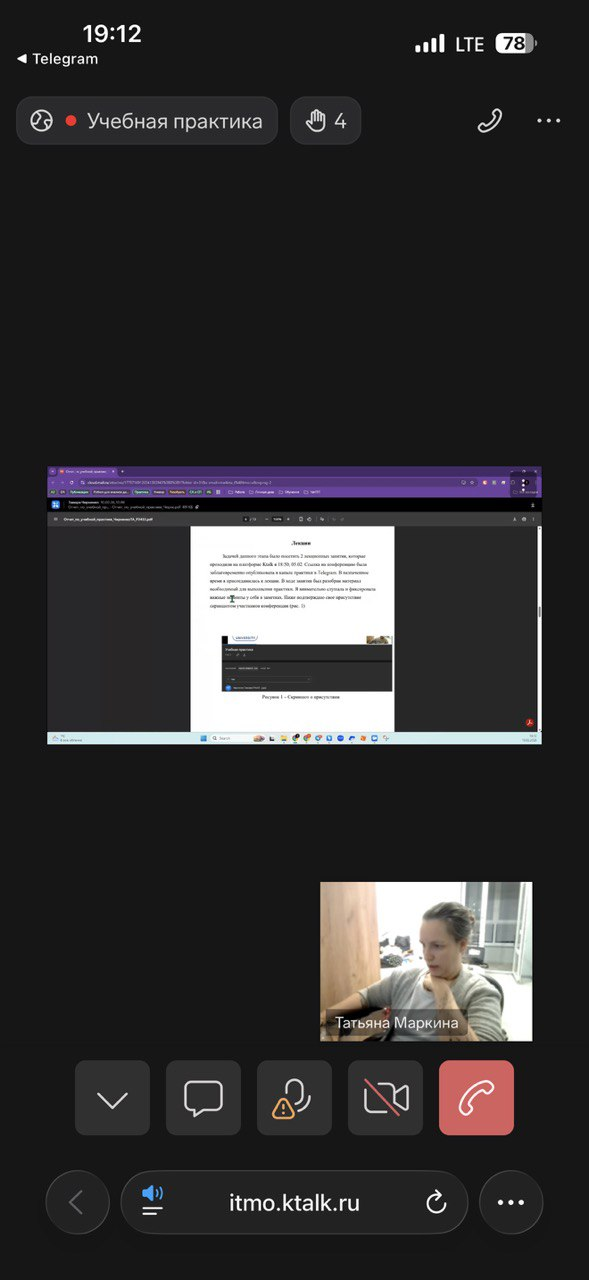
\includegraphics[height=0.55\textheight]{2.jpg}
  \caption{Скриншот присутствия на консультации}
\end{figure}

\newpage

% === ПРИЛОЖЕНИЕ Б ===
\phantomsection
\begin{flushright}
ПРИЛОЖЕНИЕ Б
\end{flushright}
\addcontentsline{toc}{section}{ПРИЛОЖЕНИЕ Б}

\begin{center}
\textbf{Техническое задание по ВКР}
\end{center}

\vspace{0.5cm}

\includepdf[pages=-]{tz.pdf}

\end{document}
